\documentclass[11pt,a4paper]{article}

\usepackage[margin=2.2cm]{geometry}

\usepackage{booktabs}
\usepackage{tabularx}
\usepackage{enumitem}
\usepackage{titlesec}
\usepackage{tikz}
\usetikzlibrary{positioning,arrows.meta,fit}
\usepackage[hidelinks]{hyperref}

\setlist{itemsep=2pt,topsep=4pt}
\titleformat{\section}{\large\bfseries}{\thesection.}{0.6em}{}
\titlespacing*{\section}{0pt}{14pt}{6pt}
\setlength{\parindent}{0pt}
\setlength{\parskip}{6pt}
\newcommand{\code}[1]{\texttt{#1}}

\begin{document}

% ---------------------------------------------------------------- Title
\begin{center}
  {\LARGE\bfseries AgPitch}\\[4pt]
  {\large Live football match insights that explain \emph{why} the game is changing}\\[10pt]
  Project Report\\[2pt]
  Roshan Palem \quad\textperiodcentered\quad October 2026
\end{center}

\vspace{4pt}
\begin{tabularx}{\textwidth}{@{}lX@{}}
\toprule
Hackathon  & Inside the Game: Developer Hackathon (Microsoft + Premier League) \\
Challenge  & The Synthetic Match Insights Engine for Premier League Studio \\
Team       & Solo \\
Live app   & \url{https://thankful-rock-0c1b05c0f.6.azurestaticapps.net} \\
Demo video & \url{https://youtu.be/Nov0eNelsuE} \\
Code       & \url{https://github.com/roshanroy7/AgPitch} \\
\bottomrule
\end{tabularx}

% ---------------------------------------------------------------- 1
\section{The problem}

When I watch a match I get the score and a few stats, but nobody tells me \emph{why} the game just turned. Why did a team suddenly start losing the ball? Was that save actually important? And a stats nerd and a casual fan want completely different answers to the same question.

The challenge asked for an engine that takes a stream of match events and turns it into live insights a broadcaster could use. My goal was simple: explain the match as it happens, and explain it differently for each viewer.

% ---------------------------------------------------------------- 2
\section{What I built}

AgPitch replays a full 90-minute synthetic match as if it were live, flags the moments that matter, and has four AI agents on Azure AI Foundry explain each one, turn it into an on-screen graphic, and rewrite it for the person watching.

\begin{itemize}
  \item Live score, clock, scorers and a commentary feed (shots, saves, blocks, corners, counter-attacks, fouls, cards, injuries)
  \item AI insight cards that appear at the exact minute of each key moment, with a ``Why it matters'' explanation
  \item Three viewing modes: casual fan, analyst and player focus
  \item Favourite club and favourite player
  \item Three languages: English, Spanish and Portuguese (every line of the interface, not just the AI text)
  \item Stats tab with top stats and a clickable shot map
  \item Full-time recap written for that viewer
  \item Changing a setting mid-match continues the stream from the current minute
\end{itemize}

% ---------------------------------------------------------------- 3
\section{Architecture}

\begin{center}
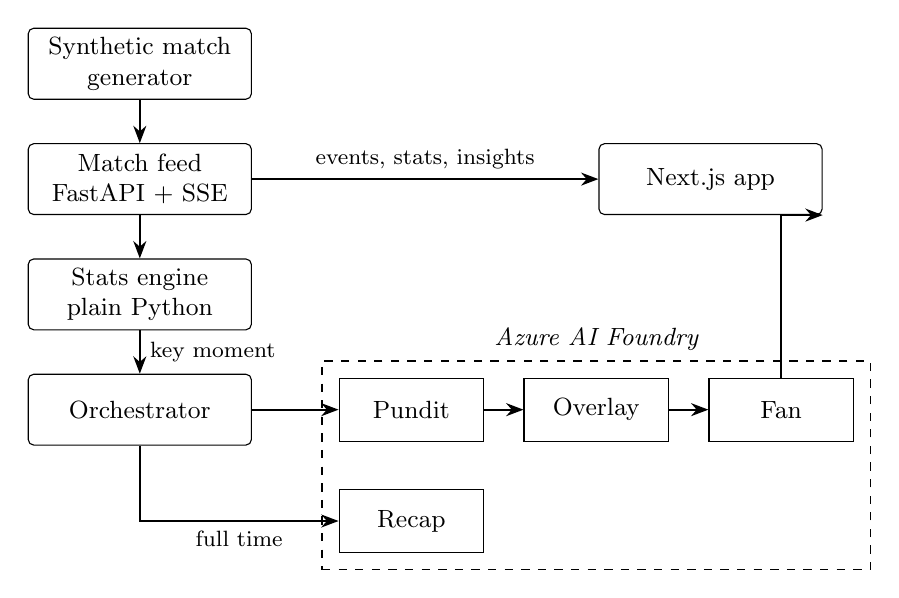
\begin{tikzpicture}[
  box/.style={draw, rounded corners=2pt, align=center, minimum height=0.9cm, text width=2.6cm, font=\small},
  agent/.style={draw, align=center, minimum height=0.8cm, text width=1.6cm, font=\small},
  arr/.style={-{Stealth[length=2.2mm]}, thick},
  node distance=0.55cm and 0.6cm]
  \node[box] (gen) {Synthetic match generator};
  \node[box, below=of gen] (feed) {Match feed\\FastAPI + SSE};
  \node[box, below=of feed] (stats) {Stats engine\\plain Python};
  \node[box, below=of stats] (orch) {Orchestrator};
  \node[agent, right=1.1cm of orch] (pundit) {Pundit};
  \node[agent, right=0.5cm of pundit] (overlay) {Overlay};
  \node[agent, right=0.5cm of overlay] (fan) {Fan};
  \node[agent, below=0.6cm of pundit] (recap) {Recap};
  \node[draw, dashed, inner sep=6pt, fit=(pundit)(overlay)(fan)(recap),
        label={[font=\small\itshape]above:Azure AI Foundry}] (foundry) {};
  \node[box, right=1.2cm of feed, xshift=3.2cm] (ui) {Next.js app};

  \draw[arr] (gen) -- (feed);
  \draw[arr] (feed) -- (stats);
  \draw[arr] (stats) -- node[right, font=\footnotesize] {key moment} (orch);
  \draw[arr] (orch) -- (pundit);
  \draw[arr] (pundit) -- (overlay);
  \draw[arr] (overlay) -- (fan);
  \draw[arr] (orch.south) |- node[below, pos=0.75, font=\footnotesize] {full time} (recap.west);
  \draw[arr] (feed) -- node[above, font=\footnotesize] {events, stats, insights} (ui);
  \draw[arr] (fan.north) |- (ui.south east);
\end{tikzpicture}
\end{center}

\begin{tabularx}{\textwidth}{@{}llX@{}}
\toprule
\textbf{Stage} & \textbf{Component} & \textbf{What it does} \\
\midrule
Ingest      & \code{main.py}       & Replays the match event by event and streams it with Server-Sent Events \\
Interpret   & \code{stats.py}      & Computes all numbers and flags key moments using rules, no AI \\
Explain     & Pundit agent         & Explains why the moment matters: control vs chaos, pressure, momentum, rhythm \\
Render      & Overlay agent        & Produces a timed, machine-readable graphic (type, headline, stat, duration, priority) \\
Personalise & Fan + Recap agents   & Rewrites the insight for the viewer's mode, club, player and language; writes the full-time recap \\
\bottomrule
\end{tabularx}

% ---------------------------------------------------------------- 4
\section{Synthetic data}

No real Premier League data is used. \code{generator.py} builds a full match (Kryptonites vs Ultras) from a scripted storyline: Kryptonites control the first half and score, Ultras switch to a high press after the break, equalise and win it late (2--1).

Around that storyline it generates possession chains, passes with pitch coordinates, shots (saved, blocked, off target), corners, clearances, counter-attacks, fouls, cards and injuries. A fixed random seed means it is the same match every run, which made testing and the demo repeatable. All teams and players are made up.

\begin{center}
\begin{tabular}{@{}lr@{\hspace{2.5cm}}lr@{}}
\toprule
Events          & 1,396 & Counter-attacks      & 6 \\
Goals           & 3     & Yellow cards         & 3 \\
Saves           & 15    & Injuries             & 2 \\
Corners         & 10    & Key moments flagged  & about 46 \\
\bottomrule
\end{tabular}
\end{center}

% ---------------------------------------------------------------- 5
\section{The stats engine}

Everything numeric is calculated in plain Python, not by the AI: possession (overall and last 10 minutes), pass accuracy, pass distance, a 0 to 10 pass difficulty rating, passes under pressure, shot speed, saves, corners, counter-attacks and cards.

Key moments are flagged by rules, each with a cooldown so the same thing is not flagged twice in a row:

\begin{itemize}
  \item \textbf{Turnover streak:} 8 turnovers in 5 minutes
  \item \textbf{Pressure spike} and \textbf{momentum swing} (an 18-point shift)
  \item \textbf{Speed alert} (33\,km/h and above) and \textbf{rocket shot} (100\,km/h and above)
  \item \textbf{Big save:} a shot of 90\,km/h or more saved
  \item \textbf{Counter-attack}, \textbf{cards}, \textbf{goals}, \textbf{quality pass}, \textbf{50-pass milestone}, half time and full time
\end{itemize}

% ---------------------------------------------------------------- 6
\section{Agent design}

All four agents run on \textbf{Azure AI Foundry Agent Service} with \textbf{gpt-5-mini}. They are created from code (\code{python -m backend.app.agents setup}), so their instructions are versioned in the repository.

\begin{tabularx}{\textwidth}{@{}lXX@{}}
\toprule
\textbf{Agent} & \textbf{Input} & \textbf{Output} \\
\midrule
Pundit  & Key moment + live stats                 & Theme, importance (1 to 5), insight \\
Overlay & Moment + Pundit analysis                & Graphic type, headline, stat, duration, priority \\
Fan     & Overlay + analysis + viewer profile     & Headline, body, stat, why it matters, tone \\
Recap   & Final stats + all moments + profile     & Title, summary, turning point, player of the match \\
\bottomrule
\end{tabularx}

Shared rules for every agent: the data is synthetic, never mention real clubs or players, only use numbers from the input, and always reply in JSON.

% ---------------------------------------------------------------- 7
\section{Key design decisions}

\begin{enumerate}
  \item \textbf{The AI never does the maths.} LLMs are bad at counting, so every number comes from the stats engine and the agents only explain it.
  \item \textbf{Only key moments go to the agents.} About 46 calls per match instead of about 1,400. Faster and much cheaper.
  \item \textbf{Shared vs personal work.} Pundit and Overlay run once per moment and are shared by every viewer. Fan runs once per moment per viewer profile, so ten viewers with the same profile cost one call.
  \item \textbf{The stream never waits for the AI.} Each moment becomes a background task. A card appears instantly in an ``Analysing'' state and fills in when the agents answer.
  \item \textbf{Caching everywhere.} Results are cached in memory and on disk, keyed by a fingerprint of the match file, so a regenerated match never reuses old insights.
  \item \textbf{Warm-up before a broadcast.} A \code{/warmup} endpoint runs the whole match through the agents in parallel (8 calls at a time), so every insight is ready exactly on time.
  \item \textbf{Fail safe.} If Azure fails, the viewer still gets a basic card from the stats engine, and the stream never breaks.
  \item \textbf{JSON in, JSON out.} The frontend never has to guess what an agent returned.
\end{enumerate}

% ---------------------------------------------------------------- 8
\section{Deployment}

\begin{tabularx}{\textwidth}{@{}llX@{}}
\toprule
\textbf{Part} & \textbf{Azure service} & \textbf{Notes} \\
\midrule
AI agents & Azure AI Foundry Agent Service & gpt-5-mini deployment \\
Backend   & Azure Container Apps           & FastAPI + SSE; Docker image built by GitHub Actions \\
Frontend  & Azure Static Web Apps          & Next.js static export \\
Auth      & Managed Identity               & No API keys in the code; \code{az login} locally \\
\bottomrule
\end{tabularx}

CORS is restricted to localhost and the deployed frontend.

% ---------------------------------------------------------------- 9
\section{Challenges and how I solved them}

\begin{itemize}
  \item \textbf{Insights arrived about 20 seconds late.} An agent chain takes 10 to 20 seconds, so cards appeared after the moment had passed. I added ``Analysing'' cards that appear at the right minute, sorted cards by match time instead of arrival time, and added the warm-up cache.
  \item \textbf{The free trial blocked the normal container build.} \code{az containerapp up} failed because ACR Tasks are not allowed on the free trial. I switched to building the Docker image with GitHub Actions, pushed it to GitHub Container Registry, and deployed that image to Container Apps.
  \item \textbf{Language quality.} I tried Telugu (my own language) first, but the output was not good enough, so I dropped it rather than ship something I would not watch myself. Spanish and Portuguese worked well. ``Why it matters'' stayed in English at first, so I added a \code{why} field to the Fan agent's output, written in the viewer's language.
  \item \textbf{Design.} My first interface did not feel like a football app. I redesigned it around tabs (Live, Stats, Recap), a match header, a settings pop-up and the two clubs' colours.
\end{itemize}

% ---------------------------------------------------------------- 10
\section{Limitations}

\begin{itemize}
  \item One synthetic match only; there is no real event feed yet.
  \item Insights for a new viewer profile take 10 to 20 seconds unless that profile was warmed up first.
  \item The translations have not been checked by native speakers.
  \item It runs as a single backend instance, sized for a demo, not for thousands of viewers.
\end{itemize}

% ---------------------------------------------------------------- 11
\section{What I would do next}

\begin{itemize}
  \item Connect a real event feed, and eventually generate events from video
  \item A momentum chart across the whole match
  \item More languages, each checked by native speakers
  \item Scale the backend out with a shared cache (for example Redis) so many instances can serve viewers
  \item Evaluate the agents' output with Azure AI Foundry evaluations
\end{itemize}

% ---------------------------------------------------------------- 12
\section{What I learned}

\begin{itemize}
  \item How to design a multi-agent system where each agent has one clear job and a strict JSON contract
  \item Why deterministic code should own the facts, and AI should own the explanation
  \item Streaming with Server-Sent Events, background tasks and caching to hide AI latency
  \item Deploying a full stack on Azure (Container Apps, Static Web Apps, Managed Identity), including working around free-trial limits
\end{itemize}

% ---------------------------------------------------------------- Stack
\section*{Tech stack}

Python 3.13, FastAPI, Server-Sent Events, \code{azure-ai-projects}, \code{azure-identity}, Azure AI Foundry Agent Service (gpt-5-mini), Next.js 16, React 19, plain CSS, Docker, GitHub Actions, Azure Container Apps, Azure Static Web Apps.

\end{document}
